\section{The observable quotient and universal factorization}
\label{sec:observablequotient}

The observation map induces a canonical representation of the distinctions retained by the interface. The representation is the quotient of \(X\) by observational equivalence. Quotient sets and their representative-independent maps are standard constructions \parencite[Chs. 8--11]{Halmos1974}; the factorization language used below follows the universal-property viewpoint \parencite{MacLaneBirkhoff1999,Leinster2014}.

\begin{definition}[Observable quotient]
The observable quotient of \(X\) relative to \(I\) is
\[
Q_I=X/{\sim_I}.
\]
The canonical class map is
\[
q_I:X\to Q_I,
\qquad
q_I(x)=[x]_I.
\]
\end{definition}
The quotient discards the identities of states inside each fiber and retains the partition induced by observation. It is neither larger nor smaller than the available distinctions in the following sense.

\begin{proposition}[Quotient equality]
For \(x,y\in X\),
\[
q_I(x)=q_I(y)
\quad\Longleftrightarrow\quad
x\sim_I y.
\]
\end{proposition}

\begin{proof}
Two quotient classes are equal exactly when their representatives are related by the defining equivalence relation. Here that relation is equality of observations.
\end{proof}
Let \(\im(\pi)\subseteq O\) denote the reachable observation range. Each quotient class has one observation value, and each reachable observation value has one quotient class.

\begin{theorem}[Canonical equivalence with the observation range]
The map
\[
\Phi:Q_I\to\im(\pi),
\qquad
\Phi([x]_I)=\pi(x),
\]
is well defined and bijective.
\end{theorem}

\begin{proof}
Well definedness follows because representatives of one class have equal observations. Surjectivity follows from the definition of \(\im(\pi)\). For injectivity, suppose \(\Phi([x]_I)=\Phi([y]_I)\). Then \(\pi(x)=\pi(y)\), so \(x\sim_I y\) and \([x]_I=[y]_I\).
\end{proof}
The quotient and the reachable range are therefore equivalent descriptions of accessible resolution. The quotient emphasizes which source states have been identified. The range emphasizes which observation values remain reachable.

\begin{figure}[tbp]
\centering
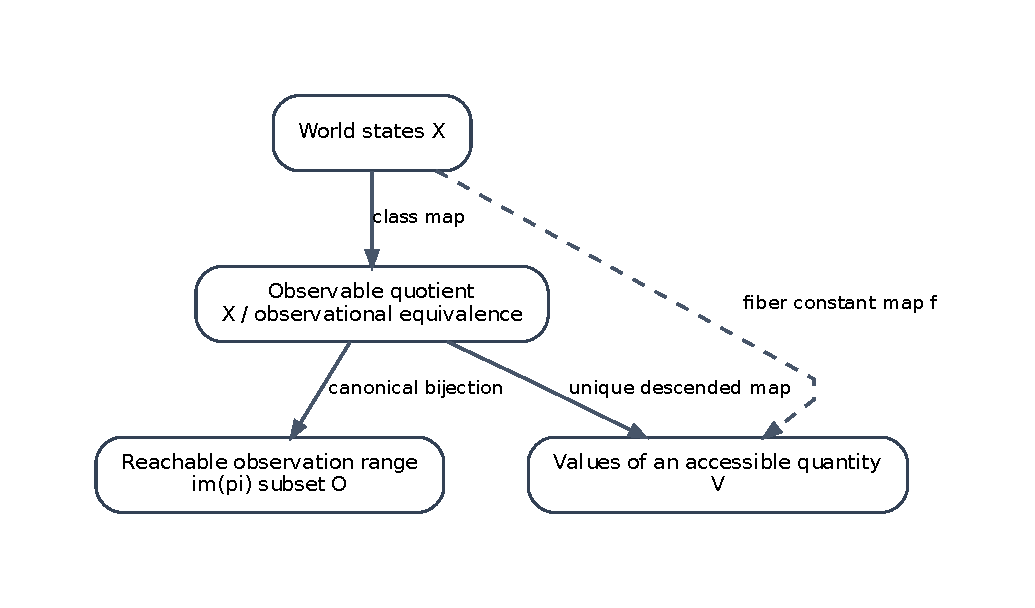
\includegraphics[width=0.88\textwidth]{figures/concept_observable_quotient.pdf}
\caption{Universal factorization through the observable quotient. A quantity defined on world states descends uniquely to the quotient exactly when it is constant on observation fibers. The quotient is canonically equivalent to the reachable observation range.}
\label{fig:observablequotient}
\end{figure}

\subsection{Universal property}

The quotient is characterized by a universal property. Universal properties identify an object by the unique maps that factor through it rather than by a choice of representatives \parencite{Leinster2014}.

\begin{theorem}[Observable quotient universal property]
Let \(f:X\to V\). The following statements are equivalent.
\begin{enumerate}[label=(\roman*)]
\item \(f(x)=f(y)\) whenever \(x\sim_I y\).
\item There exists a unique map \(\bar f:Q_I\to V\) such that
\[
f=\bar f\circ q_I.
\]
\end{enumerate}
\label{thm:observableuniversal}
\end{theorem}

\begin{proof}
Assume (i). Define \(\bar f([x]_I)=f(x)\). The definition is independent of the representative because \(f\) is constant on each equivalence class. For every \(x\in X\),
\[
(\bar f\circ q_I)(x)=\bar f([x]_I)=f(x),
\]
so the factorization exists. If \(g:Q_I\to V\) also satisfies \(f=g\circ q_I\), then for every class \([x]_I\),
\[
g([x]_I)=g(q_I(x))=f(x)=\bar f([x]_I).
\]
Thus \(g=\bar f\), proving uniqueness.

Conversely, assume (ii) and let \(x\sim_I y\). Then \(q_I(x)=q_I(y)\). Therefore
\[
f(x)=\bar f(q_I(x))=\bar f(q_I(y))=f(y).
\]
Hence \(f\) is constant on each fiber.
\end{proof}
The theorem provides a precise meaning for ``observer accessible.'' A quantity is determined on reachable observations exactly when it is a function of the observable equivalence class. Any quantity that varies inside a class requires information not present in that quotient.

\subsection{Composition with the observation range}

The original definition of interface factorization used a map \(\hat f:O\to V\). The quotient theorem uses a map \(\bar f:Q_I\to V\). These formulations agree on reachable observations. Extension to all of \(O\) is automatic when \(V\neq\varnothing\), by choosing a value on unreachable observations. If \(V=\varnothing\), a map \(X\to V\) requires \(X=\varnothing\); a map \(O\to V\) then exists only if \(O=\varnothing\). A function on the full codomain \(O\) may assign arbitrary values to unreachable observations, while a function on \(Q_I\) contains only empirically realized classes. The distinction becomes useful at the model level, where the empirical quotient is represented exactly by realizable reachable sets.
